% Drawing 142/02-12 -- folder 142, batch 02, archive page 37 (PDF page 38).
% Transcription: seconde sphère, au crayon : les deux pôles reliés par trois méridiens, les trois points marqués sur l'équateur. Légende : $\mathrm{VIII} = \mathrm{IV}$.
% Kind: sphere with poles and meridians. Method 2 (schematic redraw from the facsimile). Status: ok.
% Notes: All in faint pencil: outline, equator, the two poles joined by three meridians (one in front, two near the outline), the three marked points on the equator. The legend VIII = IV is text, not drawn.
% Coordinates: 1 unit = 1 mm = 1/100 of the crop width (bbox in page fractions: [0.18, 0.6, 0.34, 0.71]).
% Redrawn by Claude (claude-opus-5-5), issue #73, 2026-11-07; not checked by a human; not compiled (no TeX in the session).
% Rights: reproduces part of the work -- behind RENDER_TRANSCRIPTS, never published by itself.
\documentclass[tikz,border=3pt]{standalone}
\usepackage{amsmath,amssymb}
\usetikzlibrary{patterns,arrows.meta}
\tikzset{pencil/.style={black!45}, struck/.style={black!35}, mark/.style={circle,draw,inner sep=1.3pt}, pt/.style={circle,fill,inner sep=0.9pt}, opt/.style={circle,draw,fill=white,inner sep=1.1pt}}
\begin{document}
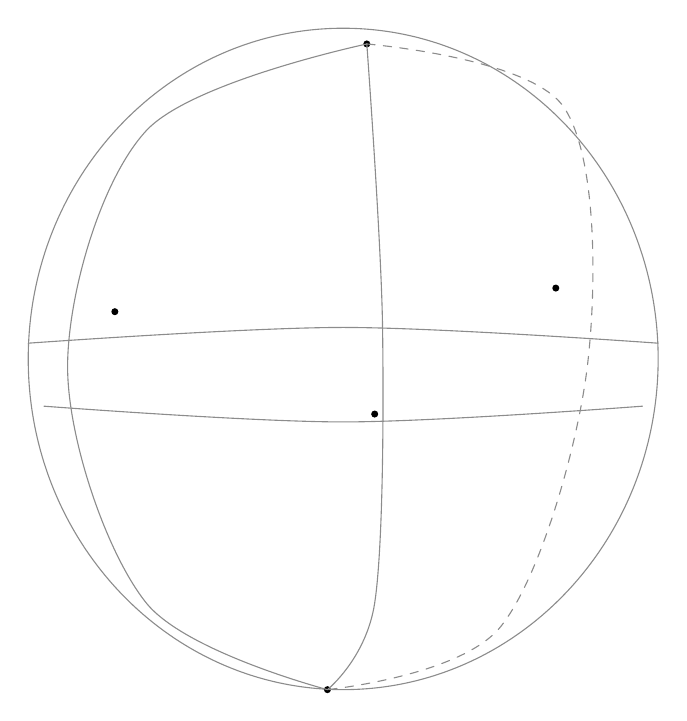
\begin{tikzpicture}[x=1mm,y=1mm,line cap=round,line join=round,font=\scriptsize]
\draw[pencil] (60,-54) ellipse[x radius=40, y radius=42];
\draw[pencil] plot[smooth, tension=0.55] coordinates {(20,-52) (60,-50) (100,-52)};
\draw[pencil] plot[smooth, tension=0.55] coordinates {(22,-60) (60,-62) (98,-60)};
\node[pt] at (63,-14) {};
\node[pt] at (58,-96) {};
\node[pt] at (31,-48) {};
\node[pt] at (64,-61) {};
\node[pt] at (87,-45) {};
\draw[pencil] plot[smooth, tension=0.55] coordinates {(63,-14) (65,-50) (64,-85) (58,-96)};
\draw[pencil] plot[smooth, tension=0.55] coordinates {(63,-14) (35,-25) (25,-55) (35,-85) (58,-96)};
\draw[pencil,dashed] plot[smooth, tension=0.55] coordinates {(63,-14) (88,-22) (91,-55) (80,-88) (58,-96)};
\end{tikzpicture}
\end{document}
